%
\section{Image Tree Based on Wordnet}
\label{sec_wordnetsearchtree}

\subsection{Wordnet}\index{Wordnet}
The offical web page (ref: http://wordnet.princeton.edu/) describes WordNet as a freely and publicly available "large lexical database of english nouns, verbs, adjectives and adverbs, grouped into sets of cognitive synonyms (synsets), each expressing a distinct concept." That is, a synset is a particular concept, that can be expressed by different terms but has one unique identifier. The identifier consists of of the word most commonly used to describe the concept, the part of speech, and a number, e.g. \emph{drive.v.02}.
The number is necessary because one word can have multiple meanings that will then be represented by different synsets, like in \emph{cherry.n.01} for the tree and \emph{cherry.n.02} for the fruit. \\

Synsets are linked with each other through several semantic relations, e.g. hyponyms or meronyms. \\
In our work, we use this network of synsets to discover the semantics between terms describing the images as well as towards the search term. \\
  

\subsection{Constructing a Searchtree}
two typical types of queries: more or less generic object descriptors, and places \\
actually construct multiple searchtrees if more than one synset found for a searchterm (i.e. train coach and motorized vehicle for car)\\
use hyponym relation to span tree of specializations (i.e. apple, banana for fruit; bus, sportscar for car)\\
if no hyponyms (usually the case for geographic terms), use part-meronyms\\
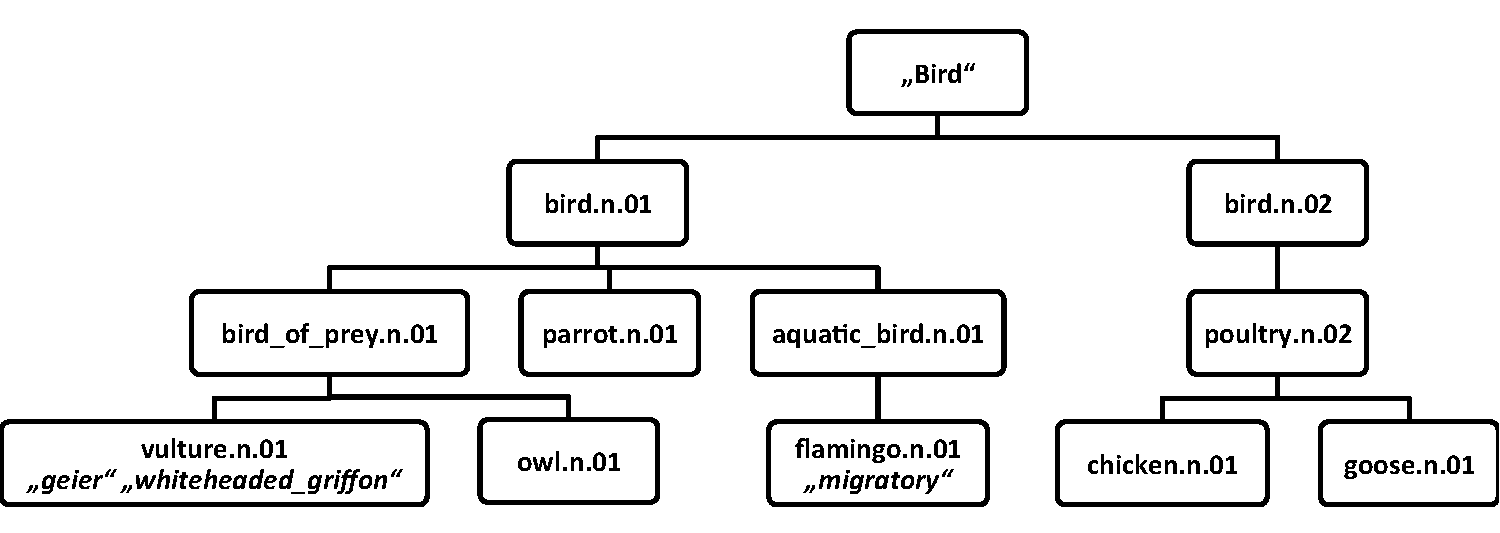
\includegraphics[width=\textwidth]{images/searchtree.pdf}

\subsection{Synset Detection}
for each tag and word in title, try to find synset (limiting ourselves to nouns, because they are usually the ones describing the depicted concepts). Further source options: description (named entity recognition necessary), comments (noticed little relation to picture), group and album names (for both preprocessing needed to match any to wordnet)  \\
problem: multiple possible synsets for a word, how to find correct meaning? \\
use best-first search (with limited queue for complexity reasons. idea is that paths at more than position x are unlikely to become best candidate anyways) \\
still erroneous with words that are meant in a way that is unknown to WordNet, i.e. canon as the camera model is interpreted as [definition of canon.n.01]  \\
therefore preprocessing removes all tags that include numbers. Blacklist could filter even more but would also filter canon in its real sense, and generally not desirable to be flexible with respect to the tag vocabulary.  \\
also removes special characters (more likely to be found on WordNet, and more likely to be identical with other unmatchable tags) 
problem: multiple possible synsets for a word, how to find correct meaning? \\
use best-first search with limited queue, distances are based on Leacock and Chodorows Normalized Path Length (lch similarities, which is perceived as closer to human understanding than regular path similarity \cite{budanitsky01} )

\subsection{Assigning Pictures to Tree Nodes}
for higher recall: find strongly co-occurring tags that could not be mapped to synset \\
strong co-occurrence defined on tf-idf (else camera models would be strong co-occurrence with many synsets)
observed that it is useful to find translations etc. but of course also introduces noise; choice of threshold (currently $0.75 * max_tf_idf$, where max tfidf is the maximal score across all values) \\
take all pictures that are annotated with at least one of the related tags or the synset itself. parameter \emph{minimal node size}: if not fulfilled, node is integrated into parent node (union pictures into parent's pictures)
